
\chapter{Stormy Clouds}

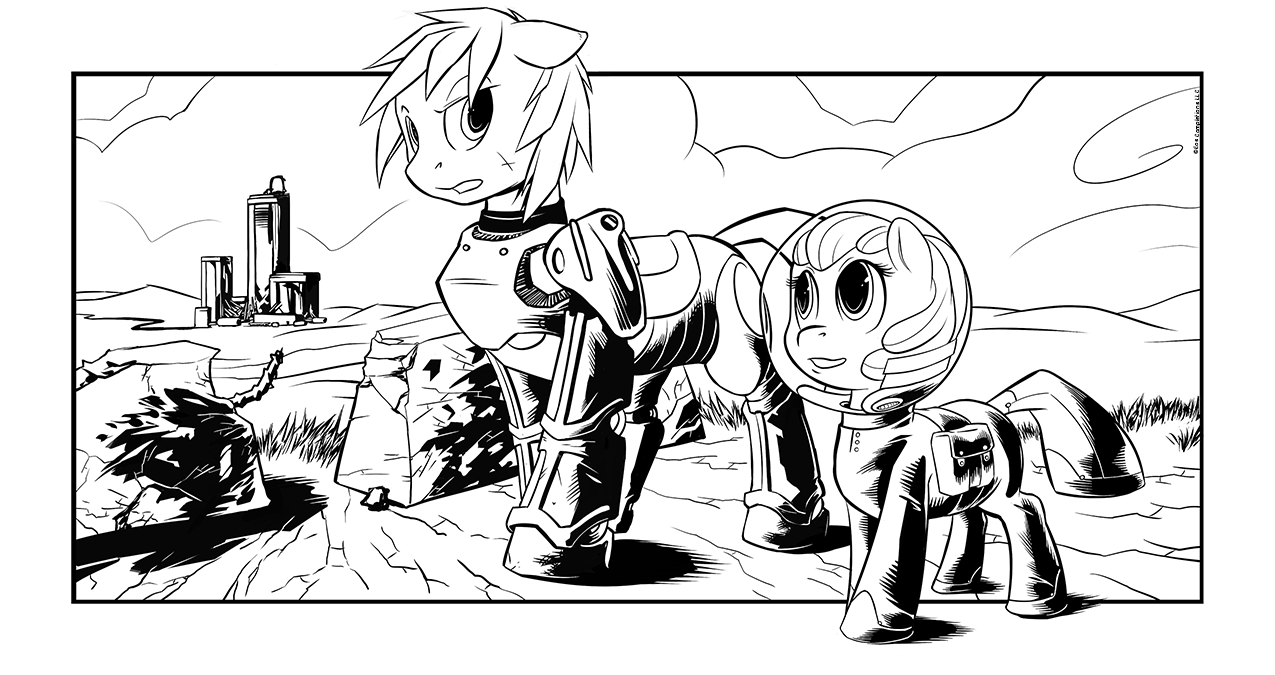
\includegraphics[width=0.9\linewidth]{image13.png}

\begin{intro}
I wanna know, have you ever seen the rain?
\end{intro}


\englishdaytimeplace{11}{18:00 P.M.}{Ivory Tower, Big 52 SC Branch}

Ivory Tower was a complex of large, white structures protected by reinforced ceramite plates. Before the war, the tower had been a research and development facility, where the Ministries of Morale and Peace worked together to find non-war oriented uses for the technological breakthroughs of the ministries of Arcane Science and Wartime Technology.

Nowadays, Ivory Tower was the only settlement on the Big 52 controlled by the Steel Rangers, mostly because it was the only place where you could find technology that hadn't been produced by Solaris Inc. And nopony with half a brain wanted to be near something made by Solaris Inc.

Yes, Solaris Inc., the company that merged a radio and a vacuum cleaner, creating the first sonic weapon ever, and putting it in the hooves of a very confused housemaid. They also invented a doorbell that incorporated a thief detection and disposal talisman, successfully electrocuting more than sixty door-to-door salesponies and a whole platoon of filly scouts selling muffins.

The central area of white buildings was surrounded by a moat and a perimeter fence, defended with automatic turrets and minefields. For more than a century, the tower held against every sort of invader, from raiders to organized war bands. Today the defenses were looking rather sorry for themselves. The turrets were destroyed and the minefields depleted. Even the perimeter fence had sustained heavy damage, having been cut in several places. The moat was crossed by two bridges, on the north and west sides of the complex, where two small collections of shacks were located. They were mostly warehouses for the caravans, and places where the traveling ponies could stay for the night and conduct business with the rangers with a roof above their heads.

The northern settlement had been almost completely razed, and the debris was used to build a barricade on the wasteland side of the north bridge, while the western group of buildings, which had been built around a couple of pre-war structures, had been hastily fortified and featured a pole with the flapping banner of the Applejack's Rangers.

The little fort was guarded by a dozen ponies, some of them still in their teens and wearing light combat saddles. A couple of fully fledged Steel Rangers in their standard power armor were guarding the bridge itself, while a third was patrolling the rocky area surrounding Ivory Tower, followed by a couple of recruits. A fourth ranger was inside the headquarters, arguing with a young mercenary.

``Yeah I can do that, no problem at all, but I want half the caps now, and some plasma stuff.'' Henrietta stretched her arms and reclined in the chair, putting her feet on the old desk.

The Ranger paladin cocked her head, a horrified expression on her muzzle. ``What do I look like, a garage sale? I'll give you a power lance, and that's already worth a fortune, but only when you're finished with the work.''

Henrietta snickered and shook her head. ``I'm a gunslinger. Don't offer me your fancy melee stuff. Three plasma grenades, two now and one later. Toss in a couple EMP mines and I'm your griffon.''

``Two EMP grenades now, a plasma grenade and a plasma mine later, last offer.'' The pony stretched her hoof towards the griffon.

Henrietta shrugged and shook the pony's leg. ``Deal. And half the caps now.''

``So you can fly away with them? I don't think so. You won't need them until you're done in any case.''

She sighed. ``You know what I think? I don't even think you have the caps. You hope that I'll accept and do the work for you, so that you can try an assault on the fort and then pay me with the caps that are inside the base. I don't think I want to play this game on the hope that four rangers and fifteen recruits will succeed in an assault against half a dozen better trained and heavily equipped ponies backed by sentries, and behind a solid defensive position.''

The paladin raised her hoof. ``All right, all right, you damn bloodwing, half the caps now! But don't expect any gratitude.''

Henri shrugged again. ``Gratitude doesn't buy bullets. I guess we have a deal. I'll be moving very soon, so be sure that your guys don't screw up.''

``All right, when you're finished, come back here and talk with Scribe Mellon. If you want to participate in the assault, I could have a little extra for you. Maybe some scavenged equipment.''

Henrietta was about to reply, when the pony in front of her held up a hoof, asking her to wait a moment. The conversation was interrupted by an emergency call for the Steel Ranger paladin.

``Cold Shower copying, report.'' The pony lowered her voice, but griffons have good hearing.

Henrietta sat in front of the desk, yawning. This wasn't her business, and she could drift away already, waiting for the night, but that thing about getting scavenged weapons from dead Steel Rangers seemed too good to be true. These ponies had to be really desperate if they made an offer like that to a griffon.

``Repeat that last part, please? You shot it dead how many times?'' The paladin's voice betrayed her disbelief. ``I don't think you can kill something more than once, Gauss.''

Henri couldn't help but turn her head toward the pony talking in the helmet, but Cold Shower was now ignoring the mercenary, immersed in her new conversation. ``What exactly do you mean by that? Are you at least sure that it's hostile?'' She paused, listening for a moment. ``So, basically, you shot it because it was creepy and it didn't even return fire?''

Henri jumped to her feet in alarm. ``Hey! Tell your guys to stop teasing Puppy!''



\horizonline

\englishdaytimeplace{11}{18:30 P.M.}{Ivory Tower, Big 52 SC Branch}

Puppysmiles trotted up to the small fort, looking at the rusty barricades and the guards on the perches. ``Hi pretty ponies! I'm Puppysmiles! Have you seen my mom?''

The glares that Puppy received in response to her greeting were mostly those of weathered ponies, tired from days of restless guard duties and broken by the awareness that they were not fighting some raiders or slavers, but ponies that they had once thought of as brothers or teachers. No, she couldn't find benevolence among this herd.

Puppy shrugged and kept narrating her interesting story to her escort. ``So, when Robocolt was sent away by the mayor, he decided to save the city all the same, because, you know, Robocolt wasn't just a robot, he was also a super kind pony!'' As usual, she didn't notice the general mood, and was already showering the poor patrol with her personal idea of what a pony with metal armor should do. ``But at that point Mom found me watching the movie and she turned off the TV.'' She shrugged. ``Meh, I can't see why she doesn't want me to watch cool movies. I mean, Robocolt is the good one. It's so obvious that in the end he'll win!''

Paladin Gauss sighed in frustration from his open helmet. ``Yes, sure, but I am NOT this Robocolt you're talking about! I'm an Applejack Ranger! It's different.''

Puppy giggled. ``You're funny, mister Not-Robocolt, I like you!''

``Yeah, whatever. Please, at least put away that dead parador! It's disgusting!'' Puppy had her pet sitting on her back. If the average pony would fear and hate such a dangerous predator, nopony could feel anything other than pity for that poor puny creature who was missing half its legs and a wing. Still, Puppy treated it like a treasure. Eww.

Puppy frowned. ``But Fuzzy Ball wants to see the pretty ponies! She will behave, I swear!''

The paladin facehoofed. ``I'm sure she will behave, but, uh, there are pet eaters around. It could be dangerous.'' He felt guilty, trying to sell her such an evident lie.

``Pet eaters? Where? Oh no, Fuzzy's in danger!'' She put the carcass of the little parador inside her saddlebags and started scouting the area in concern. ``Stay inside the bag, I'll take care of them!''

Gauss's jaw fell. He was trying to say something when one of the acolytes who had been accompanying them started laughing like an idiot, followed by the other two. Puppy stared at the laughing trio, seemingly clueless of what was going on. ``Ahahah! Very funny!'' Evidently, she didn't suspect anything.

Gauss looked away, trying to be as serious as possible. ``Right, you can never be cautious enough with those pet eaters around. Now follow me to our leader. And you three! Stop laughing like foals and report for duty at the front gates!'' He trotted away from the small group of acolytes, followed by Puppy.

``Okie dokie, Not-Robocolt! When are we going to fight crime?''

``For the last time, my name is Gauss! Paladin Gauss!'' He sighed. ``This is why I hope I'll never have foals.''

The duo finally arrived at the HQ, and Gauss opened the door, letting Puppy in before following her. The building was once a school, but now it was mostly collapsed, and all that was left were a couple of rooms and corridors that ended in a small office with white walls and a single desk in the middle. Sitting at the desk was another pony with metal armor and Henrietta.

``Henri!'' Puppy launched herself through the room, charging Henri, who effortlessly dodged the hug and caught Puppysmiles just behind the neck. Puppy struggled for a moment, trying to locate her friend. ``Hey! Where are you?''

``See? I told you that we were going to meet again.'' She put Puppy down and patted her on the helmet, snickering. ''So, Paladin, this is a friend of mine. Can you keep an eye on her while I'm doing my job?''

Cold Shower tilted her head while looking puzzled at Puppy. ``This pony was shot four times, and not only does she show no sign of it, but she's also in a good mood. I don't think I should accept her in this place until I know what I'm looking at. Gauss, call Scribe Scold.''

Puppy didn't care very much about the paladins. Now she had Henri, and this was way better. ``Yup! Mom is somewhere in the white houses on the other side of the bridge! I was going there, and I met these pretty ponies and mister Not-Robocolt!'' She finally succeeded in hugging her target. ``I'm so happy to see you again! Tell me you won't leave me alone this time!''

Henrietta cleared her voice, looking away from her. ``Uh, actually, I have a couple of things to do, but I'll be back if you wait here for me. It won't take long.''

Puppy frowned for a moment, asking uncertainly, ``Ah, will you take Silky Tail with you?''

``Sickly who? Oh, the doll! Yeah, sure, why not?''

She sighed in relief. ``Then it's all right. Just let her help you, she's good.''

Henri patted Puppy on her helmet. ``Cool, now stay with the rangers and behave. Don't make them mad, and don't run away. When I'm back I'll let you hang with me, all right?''

``Yush!'' Puppy waved goodbye to Henri as she left the room.



\horizonline

\englishdaytimeplace{11}{19:00 P.M.}{Ivory Tower, Big 52 SC Branch}

Scribe Scold was an old pony who had trained many acolytes over the years, and his cruelty and coldness toward everypony made him infamous among the young recruits. There was only one way to gain the old scribe's respect, and that was by doing a perfect job every time. When he turned against the Steel Rangers, joining the Applejack's Rangers, everypony had been surprised by his choice. In fact, a lot of the defects still thought that he was a spy.

Scold approached Puppy and looked into her eyes while talking with Paladin Cold Shower. ``Canterlot ghouls have the same scars as usual ghouls, so I don't think she's one of them.''

Cold Shower sighed, sitting behind her desk. ``Then what could this foal be? She survived four direct hits. One in the head, and three in the heart.''

``Can I has a red cape too?'' With these words Puppy grabbed Scold's cape and looked at it in amazement. ``I like the golden thingies! Gold is Pretty Princess Celestia's color! When I'm a big pony I want to be a princess too, but I need the gold! Please?''

``Runes. They're runes, and you can't \emph{have} it. Now sit down and behave.'' Scold turned back to Cold Shower. ``It could be something necromantic, I'm almost sure of that. If we had access to the library I could do some research, but at the moment I can only guess.''

``Why I can't has, ah, have it? I can give you something in exchange. It's a \emph{barter}! It's cool! Big ponies do barters every time and it's okay, not like when I changed my breakfast for two marbles and then I was really hungry and Mom scolded me! This is okay!''

Cold Shower nodded, trying to ignore Puppysmiles. ``So, what's your guess?''

Scold gave a stern look at Puppy. ``No, I don't intend to barter my cape with you. Now behave and wait until the 'big ponies' are done talking.'' He sighed before going back to Cold Shower. ``I remember reading something about these radsuits. They were less than effective during the Canterlot attack, and almost every foal wearing them was turned into a ghoul.'' Scold paused for a moment, looking at Puppy still trying to pull off his cape. ``Not this one, I'd say. Maybe I should run a diagnostic test on the suit to see what comes out.''

Scold connected his PipBuck to the data socket of Puppy's suit, keeping her still with the other leg. ``Now please stay still for a couple of minutes.''

``Can I hug you? You are funny, I like you!'' Puppy paused for a moment, pondering. ``And I like your cape, did I say that?''
>
Cold Shower couldn't help but chuckle, despite the situation. This won a grim glare from Scold. ``Yes, you can hug me as long as you stay still. Now, let's see what we have here.'' He frowned. ``It says she's deceased. No heartbeat, no body temperature. Actually, no body at all, just two thousand bone fragments and about one hundred and eighty grams of organic matter. No, it's definitely not a ghoul.''

``Tee-hee, Red Cape talks funny!''

``Yeah, Scold, stop talking funny and give me a version for the troops. Since you rejected my application as a scribe I'm more into guns than scholarship.'' There was no bad blood in Cold's words, but he occasionally needed somepony to remind him that he wasn't in his classroom.

``I still don't know. I can only say what she isn't.'' Scold looked back down at his PipBuck, reading the results of his analysis. ``The artificial intelligence of this suit is intact and working perfectly, so I'm pretty sure this is not a crazed robot. Oh, look at this. The main healing talisman failed two hundred years ago, during a reboot. A one in a thousand chance, probably caused by a short circuit or a flawed component. This activated the backup talisman.''

Cold Shower raised an eyebrow. ``And why this should be interesting?''

He snickered. ``Because the backup healing talisman had a different function to the main healing talisman.''

Cold snorted. ``Yeah, give me your information a bit at a time. Do you want to finish this thing or we are going to wait for the morning?''

Scold sighed, ignoring her comment. ``This thing doesn't seem to contain a single healing spell, just a program to manage and inoculate potions from the suit's stash. No wait, there's something else, but I don't recognize the matrix, it uses\dots zebra runes? What the hay could zebra runes be doing inside a healing talisman?''

Cold sighed and muttered, ``They could, uh, save one hundred and eighty grams of organic matter?''

He kept working with his PipBuck. ``Yes, a partially decomposed heart, I'd say. This is interesting. Scanning the inside of the suit I can see a couple of deformed high caliber bullets floating in the heart's proximity, as if they hit it without damaging the organ.'' Scold pondered for a moment. ``Let's see if I can access the registry of that talisman, then I could see how it was supposed to work.''

All this talking was plain boring. Puppy was a notoriously patient filly, but not even the most patient pony in Equestria would've been able to stand all that blah blah blah. So, she put her hooves in the scribe's pockets and started browsing through his possessions. She found a quill, some paper, a book, a pair of glasses---SNAP---uh, a monocle, another monocle. ``Hey, what's this?''

Puppy took a brushable plastic pony out of Scold's pocket. It was a green and white unicorn with a broad smile and a lyre as a cutie mark. ``D'aaw, it's so cute!'' She started petting the doll's mane. ``Brushie brushie brushie. Brushie bru---''

``What the---hey, give her back!'' He snapped the doll from Puppy's hooves, putting it back in his pocket. ``Play with your own dolls. This is an action figure, and it's very delicate and---'' Scold's eyes met Cold Shower's, and he realized what just happened. ``No, oh no, no, no no no! It's---it's a toy I confiscated from an acolyte! It's not mine!''

Puppy's eyes widened as soon as she heard that the doll hadn't a proprietor. ``Not yours? I can has that then! I'll love her and pet her and have tea with her and we will always play together and we will be best friends forever! I'm calling her Bonbon and I'll make her mane pink!''

Scold's composure evaporated when he heard about dying the doll's mane. ``Her name is Lyra and you can't HAS it! It's MI---ehr, it's confiscated material and needs to be scheduled and classified!''

An amused, evil grin appeared on Cold Shower's muzzle as she walked around the desk and trotted toward the duo. ``Oh, don't be so strict, Scribe Scold, I'm sure that we can let a little filly play with a foal's toy, right?'' Cold Shower was smiling widely, but she would have needed even more teeth to really show just how much fun she was having right now.

``See? See? Robocolt says I can has it! Gimme gimme gimme!'' She tried to pick Scold's doll again from his pockets, but this time he was on edge and blocked her.

``It's mine, okay? Lyra is mine! I can't give her to you because I like her! Are you happy now? You, ah---'' His expression changed while he looked at Cold Shower. After all, safety in mutual destruction could be an option. ``You can have a toy from the paladin's room if you wish. She will be very happy to let you rummage in her quarters, because I am sure she has nothing embarrassing to hide. Am I right, Paladin Robocolt?''

Shower's smile died as she quickly coughed and looked away. ``Ah, I'm sure we'll find some pretty toy for you, little one. Now, uh, please behave and stay put while the scribe finishes his work, okay?''

Puppy smiled in glee. A promise of new toys was good enough for her to let this funny pony with the red cloak mess with her space suit for as long as he wanted. ``Okie dokie!''

Scold sighed and launched one last accusing glare at Cold. ``Could you please stop grinning like that? I'm trying to focus here.'' He went back to his instruments, mumbling. ``Oh please, you're kidding me. They couldn't include such a feature in a healing talisman!''

Cold Shower looked puzzledly at Scold. ``What did you find? Is it as bad as it seems from your face?''

``I-I'd say it's worse. Somepony at the Ministry of Peace went to extreme lengths to make sure that these foals didn't die; that they weren't \emph{allowed} to die.''

``Weren't allowed? What do you mean by weren't allowed?'' She raised an eyebrow.

``I mean that the last resort of the backup talisman consisted of some sort of \emph{necromantic} spell. I'm not sure how it works, but it seems to bind the life of the patient to what's left of her.'' He sighed. ``Luckily enough, it doesn't seem too powerful a spell. I think it could be undone, but it will take a lot of time and study. Moreover it will require way more magical power than just my own. And I need my library.''

Cold Shower whistled. ``Talk about tough love. How could somepony do something like, like forbidding you to die? How is that even possible?'' she objected.

``Since we are facing it, I'd say it is. I'm not an expert of necromancy myself, but I can tell that the talisman itself isn't in great condition. It stayed active for two hundred years with just a single spark of energy. I can't explain it. This shouldn't work at all! There must be something else, an external factor, maybe.''

Cold tilted her head. ``So, basically, the foal is some sort of ghost?''

Scold tapped his chin. ``I'm not sure. I need to study this phenomenon a little longer. I think that the talisman somehow linked everything together. The suit, the pink goo inside it, and the remnants of the foal's body. A ghost? I don't think so, but I can't say. Technically, this poor creature shouldn't even be capable of walking around. Its magic isn't strong enough. Instead she behaves like a foal, has memories, and acts as if everything about her was normal.''

He paused for a moment, rubbing his eyes. ``Looking at this log. The suit went almost dead and didn't move at all for two centuries. Then all of a sudden its batteries got charged way above their maximum capacity, and every spell inside the suit began working at five times its effective potential. I can't explain this with science or magic. Maybe she's a ponygeist?'' With a very tired expression on his muzzle, Scold snickered and let go of Puppy's hoof. ``All right, we're finished here, little one.''

Puppy smiled back at the scribe and replied, ``Yay, now I have to go and find my mom, but I'll be back for the toys! Bye bye!''



\horizonline

\englishdaytimeplace{11}{19:45 P.M.}{Ivory Tower, Big 52 SC Branch}

Puppy pouted, looking at the closed door. ``But I have to go find my mom! I can't stay here!'' She banged at the door, but nopony answered her. She was trapped inside the classroom.

Those stoopid Robocolts put her in a room, luring her with the promise of toys, and now she was sitting in some sort of kindergarten, prisoner of those meanie ponies. Well, they actually gave her some dolls and a lot of crayons, and even a super nice coloring book, but she had no time for this! She had to find her---``Oh look, this picture has butterflies!'' No, Puppy! You must resist! You have\dots to find\dots ``Woah, a golden crayon! It's actually the color of gold! I can color Pretty Princess Celestia with this, and she will be super identical to the real one!''

No! Mom comes first! Puppy was a filly on a mission! She put down the super cool crayons and looked away. These fancy things won't keep her down! Never! ``Is that\dots a \emph{real} teapot, with \emph{real} tea cups?'' Puppy lost her battle.

Not even five minutes later, the situation was critical again. ``\emph{GASP!} Miss Fuzzy Ball ruined Rarity's gala dress, and if they don't find a gold crayon the whole gala will be spoiled! But look! Here comes Pretty Princess Celestia with a gold crayon! And there's Rainbow Dash, too! The gala is saved, yay! Now it's time to celebrate with a good cup of tea!'' Puppy was moving the dead parador and some other dolls around, talking to herself with a very focused expression on her muzzle. It was clear that she couldn't be distracted, since the gala was completely depending on that tea party.

Scold moved away from the window, shrugging. ``It seems that she won't be a problem. Keep a couple of acolytes at the door, just in case something happens, and get back to tonight's assault preparations.''

Cold Shower shivered, following the scribe. ``She seems so\dots oblivious. What should we do with her? It doesn't seem right to keep her prisoner like that, and sooner or later she will try to go and find her mother again.''

Scold sighed. ``I think I can dispel her curse. The spell is weak enough, but I must study the ritual, and I'll need other unicorns.''

``But, will she die?'' The concern in Cold's voice was evident.

Scold replied slowly, talking deliberately as if he tried to explain a very easy but vital concept to a simple mind. ``She's already dead, Cold. That little pony deserves her eternal rest. She shouldn't even exist.''

``But, she doesn't seem to care. We could at least try to see if her mother is still alive. Maybe she's a ghoul! If she lived here, there could be some information about her in the library.''

He shrugged. ``Which brings us back to our original problem: getting back my library. So, put a couple of acolytes guarding the room and start the preparations for tonight. When I have the instruments, we will discuss how to solve this problem.''



\horizonline

\englishdaytimeplace{11}{22:00 P.M.}{Ivory Tower, Big 52 SC Branch}

A little more pink in the clouds, aaand\dots done! Puppysmiles looked amazed at her new creation. Who said that you couldn't paint a picture using only pink? Pink went with everything! Now, she just needed to stick it to the wall with the others---\emph{BOOM!}

The windows shook, and for a moment there was a big red flash outside, making Puppy turn on her tail and stare in curiosity. ``Fireworks?''

\emph{BOOM!}

Another red light flared outside, and a window shattered, launching glass shards all around the room. Sharp window fragments rained on the floor, on the desks, and against Puppy's helmet. She didn't care. Instead, she stuck her head outside to get a better look at whatever was happening.

``Yay, fireworks!'' Lucky Puppy, this was a great show! Past the bridge, on the other side of the moat, a lot of ponies were running and playing, throwing fireworks and a lot of other noisy and colored lights to each other. For sure, these robocolts knew how to party hard, and Puppy wanted her share of fun.

She headed for the door, but she remembered that it was closed. Obviously this didn't discourage Puppy. She simply jumped through the window.

Landing on the road outside, Puppy hesitated. Leaving behind all those toys and pretty drawings was not easy, but everypony has to make sacrifices in order to follow their goals. What did Soft Air say? One day she would have to make sacrifices and find that not everything was easy, and you have to leave something of yours behind if you want to go on. Puppy now knew that the ugly pony was right, and Trigger Happy too, but she was a filly on a mission, and she wanted to see the fireworks from closer, so, goodbye, pretty toys. Oh, and she still had to find Mom! Finding Mom was important, too! Go Puppy!



\horizonline

\englishdaytimeplace{11}{22:15 P.M.}{Ivory Tower, Big 52 SC Branch}

The whole area between the bridge and the main research building entrance had become a battlefield. The four Applejack Rangers were supporting the attack with their heavy weapons, but the real assault was performed by the acolytes, protected only by light armor, and armed with light caliber weapons like assault rifles and submachine guns. When Puppy crossed the bridge, Paladin Gauss didn't notice her immediately and she slipped past him before he could react.

``Fuck, what is she doing here? Shower, the ghost is on the field!'' He tried following Puppy, but he had to dive behind cover again when a barrage of bullets hit his position. ``No can do! If I move I'm dead! Moreover, group two needs cover!''

Puppy noticed a young mare lying beside a smoking crater. As she approached, she could see that a pool of red had formed beneath the sleepy pony and that it was continuing to grow. ``Hey, is something wrong pretty pony?'' Puppy poked the acolyte, who weakly opened an eye.

``P-please\dots Help me\dots I\dots I don't want to die\dots'' The soldier's voice was feeble, and she couldn't even move.

Puppy gently patted the acolyte's mane. ``Don't worry, fireworks can be a little scary, but you are a big pony, so you don't have to cry.''

The dying pony stared up at her blankly, not even hearing the foal's comforting words. ``I\dots don't want to\dots die\dots'' She was a young mare, probably a fresh recruit at her first and last battle.

``There, there.'' Puppy sat down next to the pony, continuing to stroke her mane. ``I'm here, don't worry, there's nothing to be scared of. When the fireworks end we will go and buy cotton candy, okie dokie?'' The first time Puppy saw fireworks she was scared too, but Mom bought her cotton candy and she stopped crying. It must have worked with this pony, because she stopped whimpering and now she was simply crying. A couple of bullets hit Puppy in the torso while she sat beside the mare, but she hardly noticed.

``Mom\dots Sorry\dots Why I\dots ran away?'' The acolyte's dying words were barely a whisper as her last breath left her lips.

``Uh, don't worry miss pretty pony, moms are good and nice. She will be happy to see you again even if you ran away. Ah, maybe she will scold you, but I'm sure she cares.'' The dead pony didn't reply, so Puppy tried poking her. ``Ah, are you all right? Miss pretty pony? Ah, Mister Voice, is this pony all right?''

{\mten ``Analyzing. Negative. Applejack Rangers Acolyte condition: deceased.''}

Puppy frowned. ``Oh, like Henri's dad.'' Finally, Puppy seemed to catch up with the situation. ``Hey, Mister Voice, are these ponies playing or fighting?''

{\mten ``The ponies in the area are fighting, though none of them are marked as hostile toward you. Only point defenses are marked as enemies.''}

To reinforce the suit's words, another couple of bullets hit near Puppy's position, and one partially cracked her helmet.

{\mten ``Warning. Breach in the containment layer. Repair talisman activated. Hostile count: two.''}

``Hey! Look where you point those things!'' Puppy stood on her hooves, leaving the dead pony and trotting toward the nearest group of acolytes who had found shelter behind an upturned cart. ``Stop fighting! It's dangerous! Your friend is very ill!''

One of the three soldiers stared at Puppy. ``What the fuck are you doing here, filly? Find some cover!''

She tilted her head, confused. ``Why?'' Exactly at that moment, a spray of bullets hit Puppy's flank, leaving a thin trail of pink when the bullets pierced her body as if she had been made of butter.

The acolytes stared at the scene in horror, but when Puppy simply yelled at the turret to stop being a bully, they seemed speechless. The trio of soldiers didn't even react when she lost it and galloped toward the Steel Ranger's most advanced defensive position.

``Stop that! It's dangerous, stoopid bullies! Can't you see that everypony is scared here?'' Puppy charged directly toward the main building entrance, where a couple of Steel Rangers were shooting at the assailing forces.

One of the rangers turned toward her and shot at her with grenade launcher, sending her flying over to the other side of the battlefield. Puppy took a minute to recover from the explosion, and in the meantime Paladin Cold Shower managed to reach her.

``What the hay are you doing here, Puppy? Go back in the school building!''

Puppy sat down, shaking her head. ``Nope, I don't like ponies arguing with each other. Ponies should be pretty and nice, not mean and violent!''

Cold cocked her head. ``This is war, Puppy! You can't stop it by just whining! We'll handle this one. Don't worry and run back to the school. It's too dangerous here!''

``Ah! There is no war that Space Captain Andromeda can't stop!'' She lifted one hoof and stated, ``Lazer Gun!'' Sentenza floated in front of her.

Shower tried grabbing Puppy, but a burst of bullets forced her to get back into cover. ``Put away that toy gun and come with me! Puppy! Are you listening to me? Puppy!''

She galloped into the middle of the battlefield, grabbing the gun with both her hooves and pointing it at the ponies defending the main building entrance. ``Stop fighting and surrender or I'll shoot! You are bad ponies, and you should feel bad!''

A turret hit Puppy in a leg and in the belly while the rangers ignored them. Cold Shower desperately looked for an opening in the barrage of fire to dart in and grab her.

``Okie. Dokie. Lokie. Space Captain Andromeda, to the stars and beyond!'' She dived onto the ground as if she was dodging invisible laser rays and pointed her own ``toy'' gun, before stating a single word.

``Bang!''

Half a dozen times.

``Bang! Bang! Bang bang! Bang! Surrender nao, stoopid zebra aliens!''

{\mten ``Target one to seven acquired. Opening communication bridge to Ponymedes through Comm Station two. Ponymedes status: restored and functional. Relaying coordinates.''}

A window on the third story of the central building exploded from the inside, and a griffon flew out of it, firing a pistol back into the room she just left. The griffon's appearance on the battlefield completely gained Puppy's attention.

{\mten ``Ponymedes I, IV, V, IX, X and XII are ready to fire. Ponymedes II, III, VI, VII and VIII have target beyond their horizon. Relocating for indirect fire. Estimate time: 30 seconds.''}

% NOTE: force to break line

``Henri! HEEENRIII! I'm here! Make these ponies stop fighting please! HEY! HENRI!'' Puppy tried to gallop after Henri, with Sentenza still in one hoof and a turret stubbornly firing at her. ``WAAAA-AIT!''
% ``Henri! HEEENRIII! I'm here! Make these ponies stop fighting please! HEY! HENRI!'' Puppy tried to gallop after Henri, with Sentenza still in one hoof and a turret stubbornly firing at her. ``WAAAAAIT!''

Stoopid chicken, that girl always needed some help to notice things! Puppy put away the gun and took a chunk of asphalt from the ground, taking aim aaand---bull's eye! Henri lost control of her trajectory and landed, well, crashed, not far away from Puppy.

In the darkness of night, Ponymedes opened its eyes. Half a dozen red lights pointed at the roof of the base's main building. At first they were only pale, thin, crimson lines moving randomly in the area, but they grew in intensity until you could see them even from the other side of the bridge. Like red laser beams, they appeared from the clouds, piercing the gray curtain and coloring it with faint red shadows, seven small pillars of light connecting Ivory Tower with the heavens, and beyond.

``EVACUATE THE AREA! ALL PONIES LEAVE YOUR POSITION AND RETREAT!'' Enhanced with magic, Scold's voice thundered above the explosions. Every acolyte began falling back, following Scold's order, leaving their cover and running toward the bridge. The rangers defending the central building seemed confused, and held their fire as they watched the retreating forces.

``Fuck, Puppy, why did you throw a stone at me this time?'' Henrietta was rubbing her head, still trying to work out what was happening. ``What's the old mummy screaming?''

Puppy shrugged and hugged her friend. ``Dunno, but I wanted you to tell them to stop being mean, only it seems that they are already stopping.''

{\mten ``All weapons ready to fire. Target is locked. Commencing full scale attack in ten\dots nine\dots''}

~\vfill

\begin{engnote}
		Level up! (12)
	
		New perk added: Little Scoundrel - No Puppy, give it back! You are less likely to get caught when stealing, in addition you can access to NPC's inventory during dialogues if you are facing them.
\end{engnote}

